\appendix
\chapter{Dodatak}


��  ��   ��  ��  �� nj

\listoffixmes

\newpage

\subsection*{Brlja}

\begin{exerciseslots}
\hspace{1cm}
\= \exslot{aaa}
\= \exslot{bbb}
\\
\> \exslot{ccc}
\> \exslot{ddd}
\\
\> \exslot{eee}
\> \exslot{fff}
\\
\> \exslot{ggg}
\> \exslot{hhh}
\end{exerciseslots}


\value{innerexample}

\begin{rj}[Konj]  \mbox{}
  \begin{enumerate}
    \item prvi
    \item drugi
  \end{enumerate}
\end{rj}

\begin{innerexample}
   \mbox{}
  \begin{enumerate}
    \item prvi
    \item drugi
  \end{enumerate}
\end{innerexample}

\begin{rj}
\item[] nesto sam htio reci
\item[] jos nesto sam htio reci
\end{rj}

\begin{example}
\item[] nesto sam htio reci
\item[] jos nesto sam htio reci
\end{example}

\begin{rj}
\item[]
  d flaksjd lfkajsl dkfj lsdkjf slkdjf alksjd flksdj fa lsdkjf
slkdjf alksjd flksdj faBrlajalksdj laskdj flaksdj flaksjd flaksjd
flaksjd lfkajsl dkfj lsdkjf slkdjf alksjd flksdj fa Brlajalksdj
laskdj flaksdj flaksjd flaksjd flaksjd lfkajsl dkfj lsdkjf slkdjf
alksjd flksdj fa
\end{rj}

\begin{example}
\item[]
  Primijetimo da je $y=x^3$ rje\v{s}enje  podru\v{c}ju realnih brojeva
podru\v{c}ju realnih brojeva Primijetimo da je $y=x^3$
rje\v{s}enje  podru\v{c}ju realnih brojeva podru\v{c}ju realnih
brojeva
\end{example}

\begin{example}\label{pr 2.1}
Primijetimo da je $y=x^3$ rje\v{s}enje  podru\v{c}ju realnih brojeva
podru\v{c}ju realnih brojeva


podru\v{c}ju realnih brojeva
podru\v{c}ju realnih brojeva
podru\v{c}ju realnih brojeva
\begin{enumerate}%[\indent a)]
 \item Provjerimo da je $y=x^3$ rje\v{s}enje jednad\v{z}be $xy'=3y$
 na \v{c}itavom podru\v{c}ju realnih brojeva.
 \item Provjerimo da je $x_2+y_2=1$ implicitno rje\v{s}enje jednad\v{z}be $yy'=-x$ na
 intervalu $(-1,1)$.
  \item Provjerimo da je $x_2+y_2=1$ implicitno rje\v{s}enje jednad\v{z}be $yy'=-x$ na
 intervalu $(-1,1)$.
 \begin{enumerate}%[\indent a)]
 \item Provjerimo da je $y=x^3$ rje\v{s}enje jednad\v{z}be $xy'=3y$
 na \v{c}itavom podru\v{c}ju realnih brojeva.
  \begin{enumerate}%[\indent a)]
 \item Provjerimo da je $y=x^3$ rje\v{s}enje jednad\v{z}be $xy'=3y$
 na \v{c}itavom podru\v{c}ju realnih brojeva.
 \item Provjerimo da je $x_2+y_2=1$ implicitno rje\v{s}enje jednad\v{z}be $yy'=-x$ na
 intervalu $(-1,1)$.
  \item Provjerimo da je $x_2+y_2=1$ implicitno rje\v{s}enje jednad\v{z}be $yy'=-x$ na
 intervalu $(-1,1)$.  \begin{enumerate}%[\indent a)]
 \item Provjerimo da je $y=x^3$ rje\v{s}enje jednad\v{z}be $xy'=3y$
 na \v{c}itavom podru\v{c}ju realnih brojeva.
 \item Provjerimo da je $x_2+y_2=1$ implicitno rje\v{s}enje jednad\v{z}be $yy'=-x$ na
 intervalu $(-1,1)$.
  \item Provjerimo da je $x_2+y_2=1$ implicitno rje\v{s}enje jednad\v{z}be $yy'=-x$ na
 intervalu $(-1,1)$.
\end{enumerate}
\end{enumerate}
 \item Provjerimo da je $x_2+y_2=1$ implicitno rje\v{s}enje jednad\v{z}be $yy'=-x$ na
 intervalu $(-1,1)$.
  \item Provjerimo da je $x_2+y_2=1$ implicitno rje\v{s}enje jednad\v{z}be $yy'=-x$ na
 intervalu $(-1,1)$.
\end{enumerate}
\end{enumerate}
\end{example}

\begin{innerexample} Foxy gralkjs sldkfjs dfls dflkasjd
\end{innerexample}


\begin{list}{}{}
\item[]
\begin{theorem}    \ asdf
  \begin{enumerate}%[\indent a)]
 \item Provjerimo da je $y=x^3$ rje\v{s}enje jednad\v{z}be $xy'=3y$
 na \v{c}itavom podru\v{c}ju realnih brojeva.
 \item Provjerimo da je $x_2+y_2=1$ implicitno rje\v{s}enje jednad\v{z}be $yy'=-x$ na
 intervalu $(-1,1)$.
  \item Provjerimo da je $x_2+y_2=1$ implicitno rje\v{s}enje jednad\v{z}be $yy'=-x$ na
 intervalu $(-1,1)$.
\end{enumerate}
\end{theorem}
\end{list}

\begin{proposition}
          \ asdf              \begin{enumerate}%[\indent a)]
 \item Provjerimo da je $y=x^3$ rje\v{s}enje jednad\v{z}be $xy'=3y$
 na \v{c}itavom podru\v{c}ju realnih brojeva.
 \item Provjerimo da je $x_2+y_2=1$ implicitno rje\v{s}enje jednad\v{z}be $yy'=-x$ na
\end{enumerate}
\end{proposition}

\begin{enumerate}%[\indent a)]
 \item Provjerimo da je $y=x^3$ rje\v{s}enje jednad\v{z}be $xy'=3y$
 na \v{c}itavom podru\v{c}ju realnih brojeva.
 \item Provjerimo da je $x_2+y_2=1$ implicitno rje\v{s}enje jednad\v{z}be $yy'=-x$ na
 intervalu $(-1,1)$.
  \item Provjerimo da je $x_2+y_2=1$ implicitno rje\v{s}enje jednad\v{z}be $yy'=-x$ na
 intervalu $(-1,1)$.
\end{enumerate}



\begin{enumerate}%[\indent a)]
 \item Provjerimo da je $y=x^3$ rje\v{s}enje jednad\v{z}be $xy'=3y$
 na \v{c}itavom podru\v{c}ju realnih brojeva.
 \item Provjerimo da je $x_2+y_2=1$ implicitno rje\v{s}enje jednad\v{z}be $yy'=-x$ na
 intervalu $(-1,1)$.
  \item Provjerimo da je $x_2+y_2=1$ implicitno rje\v{s}enje jednad\v{z}be $yy'=-x$ na
 intervalu $(-1,1)$.
\end{enumerate}

%\begin{exm}
%  Primjercic
%flaksjd flaksjd flaksjd lfkajsl dkfj
%Brlajalksdj laskdj flaksdj flaksjd flaksjd flaksjd lfkajsl dkfj
%lsdkjf slkdjf alksjd flksdj
%\end{exm}
%
%\begin{exm}[neki primjer]
%  Primjercic
%flaksjd flaksjd flaksjd lfkajsl dkfj
%Brlajalksdj laskdj flaksdj flaksjd flaksjd flaksjd lfkajsl dkfj
%lsdkjf slkdjf alksjd flksdj
%\end{exm}

\begin{example} Primjercic
flaksjd flaksjd flaksjd lfkajsl dkfj
Brlajalksdj laskdj flaksdj flaksjd flaksjd flaksjd lfkajsl dkfj
lsdkjf slkdjf alksjd flksdj fa Brlajalksdj laskdj flaksdj flaksjd
\end{example}

Brlajalksdj laskdj flaksdj flaksjd flaksjd flaksjd lfkajsl dkfj
Brlajalksdj laskdj flaksdj flaksjd flaksjd flaksjd lfkajsl dkfj
lsdkjf slkdjf alksjd flksdj fa Brlajalksdj laskdj flaksdj flaksjd
flaksjd flaksjd lfkajsl dkfj lsdkjf slkdjf alksjd flksdj fa lsdkjf
slkdjf alksjd flksdj faBrlajalksdj laskdj flaksdj flaksjd flaksjd
flaksjd lfkajsl dkfj lsdkjf slkdjf alksjd flksdj fa Brlajalksdj
laskdj flaksdj flaksjd flaksjd flaksjd lfkajsl dkfj lsdkjf slkdjf
alksjd flksdj fa

\begin{rj}
  d flaksjd lfkajsl dkfj lsdkjf slkdjf alksjd flksdj fa lsdkjf
slkdjf alksjd flksdj faBrlajalksdj laskdj flaksdj flaksjd flaksjd
flaksjd lfkajsl dkfj lsdkjf slkdjf alksjd flksdj fa Brlajalksdj
laskdj flaksdj flaksjd flaksjd flaksjd lfkajsl dkfj lsdkjf slkdjf
alksjd flksdj fa
\end{rj}

\begin{rj}
%kfj lsdkjf slkdjf alksjd flksdj fa lsdkjf
%slkdjf alksjd flksdj faBrlaj
%{
%\setlength{\topsep}{0pt}
%\begin{compactenum}
%  \item asd
%  \item baskjdfhkasjdf
%\end{compactenum}
%}
%\vspace{-1ex}
\begin{list}{}{
 \setlength{\topsep}{0pt plus 0pt minus 0pt}
 \setlength{\parsep}{0pt}
 \setlength{\partopsep}{0pt}
 \setlength{\parskip}{0pt}
 }
  \item asd
  \item baskjdfhkasjdf
 \end{list}
  d flaksjd lfkajsl dkfj lsdkjf slkdjf alksjd flksdj fa lsdkjf
slkdjf alksjd flksdj faBrlajalksdj laskdj flaksdj flaksjd flaksjd
flaksjd lfkajsl dkfj lsdkjf slkdjf alksjd flksdj fa Brlajalksdj
laskdj flaksdj flaksjd flaksjd flaksjd lfkajsl dkfj lsdkjf slkdjf
alksjd flksdj fa
\end{rj}

\begin{center}
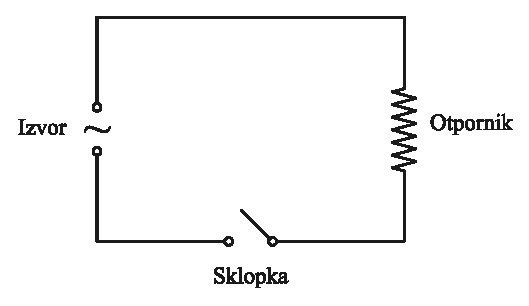
\includegraphics[width=6cm]{SL_01}
\end{center}





 \plavapozadina
{\begin{okvir}[�erivacija]
 flaksjd lfkajsl dkfj lsdkjf slkdjf alksjd flksdj fa lsdkjf
slkdjf alksjd flksdj faBrlajalksdj laskdj flaksdj flaksjd flaksjd
flaksjd lfkajsl dkfj lsdkjf slkdjf alksjd flksdj fa Brlajalksdj
laskdj flaksdj flaksjd flaksjd flaksjd lfkajsl dkfj lsdkjf slkdjf
alksjd flksdj fa


\textbf{\textsf{\emph{  ��  ��   ��  ��  �� nj  }}}
\end{okvir}}


\begin{centering}
   lfkajsl dkfj lsdkjf slkdjf alksjd flksdj fa lsdkjf
slkdjf alksjd flksdj faBrlajalksdj laskdj flaksdj flaksjd flaksjd
flaksjd lfkajsl
 lfkajsl dkfj lsdkjf slkdjf alksjd flksdj fa lsdkjf
slkdjf alksjd flksdj faBrlajalksdj laskdj flaksdj flaksjd flaksjd
flaksjd lfkajsl
\end{centering}


\medskip

 {\DJ}


\newpage

%\layout


%\input{TODO.txt}
